\documentclass[beamer]{standalone}
\usepackage{circuitikz}

\tikzstyle{block} = [draw, fill=blue!20, rectangle, 
    minimum height=3em, minimum width=6em]
\tikzstyle{sum} = [draw, fill=blue!20, circle, node distance=1cm]
\tikzstyle{input} = [coordinate]
\tikzstyle{output} = [coordinate]
\tikzstyle{pinstyle} = [pin edge={to-,thin,black}]

\begin{document}

\title[Electronics 1]{PID Feedback}

\begin{frame} 
  \titlepage
\end{frame}

\section{Lagrangians}
\begin{frame}{Lagrangians in Electronics}
\small Consider the following coupled $LC$ circuit where $I_{1,2} = dQ_{1,2}/dt$ is the current flowing in a loop of the circuit, $L$ is the inductance of the inductor, and $C$ is the capacitance of the capacitor.  By analogy to mechanical oscillators, the inductance plays the role of an inertial mass, the capacitance plays the role of a spring constant.  The kinetic energy in an inductor is $\frac{1}{2} L I^2$, the potential energy in a capacitor is $\frac{1}{2 C} Q^2$.  The voltage across an inductor is $L \frac{d I}{d t}$, the voltage across a capacitor is $Q/C$.
 \begin{center}
  \begin{circuitikz}
   \draw (0,3) to (4,3);
   \draw (0,0) to[L, i=$I_1$, l=$L$] (0,3);
   \draw (0,0) to[C, l=$C$] (2,0);
   \draw (2,0) to[C, l=$C$] (4,0);
   \draw (4,0) to[L, i=$I_2$, l=$L$] (4,3);
   \draw (2,0) to (2,1);
   \draw (2,3) to[C, l=$C$] (2,1);
  \end{circuitikz}
 \end{center}
 Determine the Lagrangian for this circuit, and show that the correct Kirchhoff equations can indeed be derived.
\end{frame}

\begin{frame}{Lagrangians in Electronics}
The Lagrangian for the system is
\begin{equation*}
 L = \frac{1}{2} L (I_1^2 + I_2^2) - \frac{1}{2 C} \left(Q_1^2 + Q_2^2 + (Q_1 + Q_2)^2\right).
\end{equation*}
The equations of motion are
\begin{eqnarray*}
 L \dot{I}_1 + \frac{1}{C} Q_1 + \frac{1}{C} (Q_1 + Q_2) & = & 0, \\
 L \dot{I}_2 + \frac{1}{C} Q_2 + \frac{1}{C} (Q_1 + Q_2) & = & 0.
\end{eqnarray*}
These are indeed the Kirchhoff equations one would find for the left loop and the right loop.
\end{frame}

\section{Proportional Feedback with Op Amps}
\begin{frame}
\frametitle{Feedback with Op Amps: Buffer, Amplifier}
\begin{figure}
	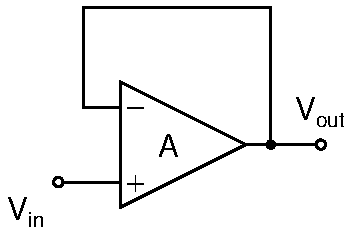
\includegraphics[width=0.30\textwidth]{./schematics/buffer.pdf}
\end{figure}
\begin{equation*}
	V_{out}=\frac{A}{A+1} V_{in}
\end{equation*}
\begin{figure}
	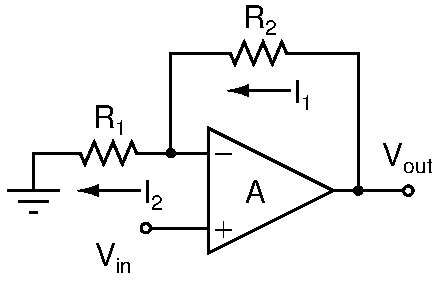
\includegraphics[width=0.30\textwidth]{./schematics/noninv_ampl.pdf}
\end{figure}
\begin{equation*}
	V_{out}=\left( 1+\frac{R_2}{R1} \right) V_{in}
	\frac{A}{A+(1+\frac{R_2}{R_1})}
\end{equation*}
\end{frame}

\section{Feedback Model}
\begin{frame}{Systems without Feedback}
 \begin{center}
  \begin{tikzpicture}[auto, node distance=2cm,>=latex']
    % http://www.texample.net/tikz/examples/control-system-principles/
    % We start by placing the blocks
    %\node [input, name=input] {};
    %\node [sum, right of=input] (sum) {};
    \node [block] (controller) {Controller};
    \node [block, right of=controller, pin={[pinstyle]above:Disturbances $v$},
            node distance=3cm] (system) {System $S$};
    % We draw an edge between the controller and system block to 
    % calculate the coordinate u. We need it to place the measurement block. 
    \draw [->] (controller) -- node[name=u] {$u$} (system);
    \node [output, right of=system] (output) {};
    \node [block, below of=u] (measurements) {Measurements};
    % Once the nodes are placed, connecting them is easy. 
    %\draw [draw,->] (input) -- node {$r$} (sum);
    %\draw [->] (sum) -- node {$e$} (controller);
    \draw [->] (system) -- node [name=y] {$y$}(output);
    \draw [->] (y) |- (measurements);
    %\draw [->] (measurements) -| node[pos=0.99] {$-$} 
    %    node [near end] {$y_m$} (sum);
  \end{tikzpicture}
 \end{center}
\end{frame}


\begin{frame}{System with Feedback}
 \begin{center}
  \begin{tikzpicture}[auto, node distance=2cm,>=latex']
    % http://www.texample.net/tikz/examples/control-system-principles/
    % We start by placing the blocks
    \node [input, name=input] {};
    \node [sum, right of=input] (sum) {};
    \node [block, right of=sum] (controller) {Controller};
    \node [block, right of=controller, pin={[pinstyle]above:Disturbances $v$},
            node distance=3cm] (system) {System $S$};
    % We draw an edge between the controller and system block to 
    % calculate the coordinate u. We need it to place the measurement block. 
    \draw [->] (controller) -- node[name=u] {$u$} (system);
    \node [output, right of=system] (output) {};
    \node [block, below of=u] (measurements) {Measurements};
    % Once the nodes are placed, connecting them is easy. 
    \draw [draw,->] (input) -- node {$y_d$} (sum);
    \draw [->] (sum) -- node {$e$} (controller);
    \draw [->] (system) -- node [name=y] {$y$}(output);
    \draw [->] (y) |- (measurements);
    \draw [->] (measurements) -| node[pos=0.99] {$-$} 
        node [near end] {$y_m$} (sum);
  \end{tikzpicture}
 \end{center}
\end{frame}

\begin{frame}{Feedback Model}
\begin{enumerate}
\item \label{enum:measure} Measure the state $S$ of the system.
\item Determine how far the system is from its desired set point by defining an error variable, $e = y_m - y_d$.
\item Calculate a trial control value $u = u(e)$.
\item Feed the calculated control value, $u(e)$, back into the control input of the system $S$.
\item \label{enum:change} The state of the system changes in response to the change in the control value.
\item Return to step \ref{enum:measure}.
\end{enumerate}
\end{frame}

\begin{frame}{Proportional-Integral-Derivative Feedback}
\begin{block}{Controller}
\begin{itemize}
\item Controls the input $u$ for the system $S$
\item We determine what input $u$ should be for a given error $e$
\end{itemize}
\end{block}
\begin{block}{PID controller}
\begin{equation}
u(e;t) = g_P e(t) + g_I \int_0^t e(t)dt + g_D \frac{d}{dt} e(t)
\end{equation}
\begin{itemize}
\item $g_P$: proportional
\item $g_I$: integral
\item $g_D$: derivative
\end{itemize}
\end{block}
\end{frame}

\section{Pure Proportional Gain Feedback}
\begin{frame}{Pure Proportional Gain Feedback}
\begin{block}{No feedback:}
\begin{equation}
S_{no~feedback}(t) = S_0
\end{equation}
\end{block}
\begin{block}{With feedback:}
Assume simplest linear system for $S$
\begin{equation}
S(t+\Delta t) = S_0 + u(e;t) = S_0 + g_P e(t)
\end{equation}
Assume characteristic time $\tau$ gives $S(t+\Delta t)$
\begin{equation}
S(t) + \tau \frac{d}{dt} S(t) = S_0 + g_P e(t) = S_0 + g_P \left(S(t) - S_d\right)
\end{equation}
\end{block}
\end{frame}

\begin{frame}{Pure Proportional Gain Feedback}
Rearrange:
\begin{equation}
(1 - g_P) S(t) + \tau \frac{d}{dt} S(t) = S_0 - g_P S_d
\end{equation}
Put in standard form for 1st order DE:
\begin{equation}
S(t) + \frac{\tau}{1 - g_P} \frac{d}{dt} S(t) = \frac{S_0 - g_P S_d}{1 - g_P}
\end{equation}
Since $y(t) e^{t/a} + a y'(t) e^{t/a} = d/dt (a y(t) e^{t/a})$:
\begin{equation}
S(t) = \left(S_0 - \frac{S_0 - g_P S_d}{1 - g_P}\right) e^{-(1-g_P)t/\tau} + \frac{S_0 - g_P S_d}{1 - g_P}
\end{equation}
\end{frame}

\begin{frame}{Pure Proportional Gain Feedback}
\begin{center}
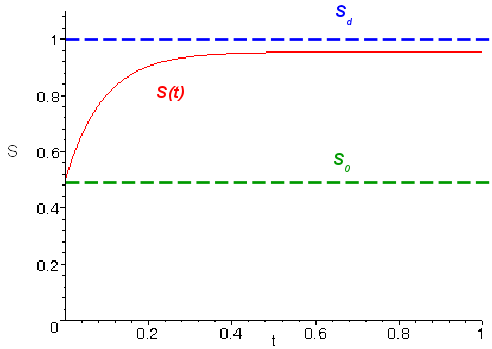
\includegraphics[width=0.7\textwidth]{pics/P_from_05_to_1}
\end{center}
System response with pure proportional gain feedback control and parameters $g_P = -10$, $S_0 = 0.5$, and $S d = 1$. Time is measure in units of $\tau$.
\end{frame}

\begin{frame}{Pure Proportional Gain Feedback}
Full solution:
\begin{equation}
S(t) = \left(S_0 - \frac{S_0 - g_P S_d}{1 - g_P}\right) e^{-(1-g_P)t/\tau} + \frac{S_0 - g_P S_d}{1 - g_P}
\end{equation}
Steady-state solution:
\begin{equation}
S_{ss} = \frac{S_0 - g_P S_d}{1 - g_P}
\end{equation}
Never reaches desired state $S_d$, but gets arbitrarily close when $g_P \to -\infty$.  Notice divergence (positive feedback) when $g_P \to +\infty$.
\end{frame}

\section{Proportional-Integral Feedback}
\begin{frame}{Proportional-Integral Feedback}
With the integral term in the control $u(e;t)$ and in the error $e(t)$:
\begin{equation}
S(t) + \tau \frac{d}{dt} S(t) = S_0 + g_P e(t) + g_I \int_0^t e(t)dt
\end{equation}
We now obtian a 2nd order differential equation:
\begin{equation}
\tau \frac{d^2}{dt^2} S(t) + (1 - g_P) \frac{d}{dt} S(t) - g_I S(t) = - g_I S_d. \label{eqn:proportional_integral_diff_eq}
\end{equation}
To determine the solutions we need the zeros $\lambda$ of the characteristic equation:
\begin{equation}
\lambda_\pm = \frac{(g_P - 1) \pm \sqrt{(g_P - 1)^2 + 4 g_I \tau}}{2 \tau}
\end{equation}
\end{frame}

\begin{frame}{Proportional-Integral Feedback}
Solution using the zeros $\lambda_\pm$:
\begin{equation}
S(t) = A_+ e^{\lambda_+ t} + A_- e^{\lambda_- t} + S_d
\end{equation}
Coefficients determined from initial conditions, e.g. $S(t=0) = S_0$ and $dS(t=0)/dt = 0$:
\begin{eqnarray}
A_+ & = & - \frac{\lambda_-}{\lambda_- - \lambda_+} (S_d - S_0), \\
A_- & = & \frac{\lambda_+}{\lambda_- - \lambda_+} (S_d - S_0).
\end{eqnarray}
\end{frame}

\begin{frame}{Proportional-Integral Feedback}
\begin{center}
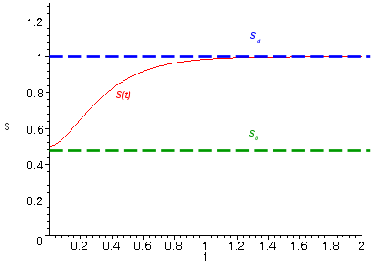
\includegraphics[width=0.49\textwidth]{pics/PI_from_05_to_1_settings1}
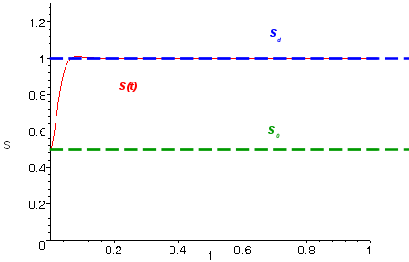
\includegraphics[width=0.49\textwidth]{pics/PI_from_05_to_1_settings2}
\end{center}
Time-evolution of a generic system with PI control feedback for $S_0 = 0.5$ and $S_d = 1$. For the left hand plot the gain parameters are $g_P = -10$, $g_I = -30$, while for the right hand plot the parameters are $g_P = -100$, $g_I = -4000$.
\end{frame}

\begin{frame}{Proportional-Integral Feedback}
The small overshoot in the left hand plot is due to a small imaginary part in the exponential exponent.

The primary purpose of integral gain is to provide essentially infinite gain at DC (0\,Hz), which guarantees that $S_{ss} = S_d$.  The larger the gain, the faster the correction time of the feedback control loop.
\end{frame}

\begin{frame}{Noise Suppression with PI Feedback}
Noise or disturbance $v$ can be modeled as $S_N \cos\omega t$, or $S_N e^{i\omega t}$.  This changes the inhomogenous right-hand side of the 2nd order differential equation.
 \begin{center}
  \begin{tikzpicture}[auto, node distance=2cm,>=latex']
    % http://www.texample.net/tikz/examples/control-system-principles/
    % We start by placing the blocks
    \node [input, name=input] {};
    \node [sum, right of=input] (sum) {};
    \node [block, right of=sum] (controller) {Controller};
    \node [block, right of=controller, pin={[pinstyle]above:Disturbances $v$},
            node distance=3cm] (system) {System $S$};
    % We draw an edge between the controller and system block to 
    % calculate the coordinate u. We need it to place the measurement block. 
    \draw [->] (controller) -- node[name=u] {$u$} (system);
    \node [output, right of=system] (output) {};
    \node [block, below of=u] (measurements) {Measurements};
    % Once the nodes are placed, connecting them is easy. 
    \draw [draw,->] (input) -- node {$y_d$} (sum);
    \draw [->] (sum) -- node {$e$} (controller);
    \draw [->] (system) -- node [name=y] {$y$}(output);
    \draw [->] (y) |- (measurements);
    \draw [->] (measurements) -| node[pos=0.99] {$-$} 
        node [near end] {$y_m$} (sum);
  \end{tikzpicture}
 \end{center}
\end{frame}

\begin{frame}{Noise Suppression with PI Feedback}
The differential equation becomes
\begin{equation}
\tau \frac{d^2}{dt^2} S(t) + (1 - g_P) \frac{d}{dt} S(t) - g_I S = i\omega S_N e^{i\omega t} - g_I S_d
\end{equation}
with solutions of the inhomogeneous part
\begin{equation}
S_{ih}(t) = \frac{i\omega}{(1 - g_P) i\omega - \tau \omega^2 - g_I} S_N  e^{i\omega t} + S_d
\end{equation}
with magnitude
\begin{equation}
A_N = \frac{\omega}{\sqrt{(1 - g_P)^2 \omega^2 + (\tau \omega^2 + g_I)^2}}.
\end{equation}
\end{frame}

\begin{frame}{Noise Suppression with PI Feedback}
\begin{center}
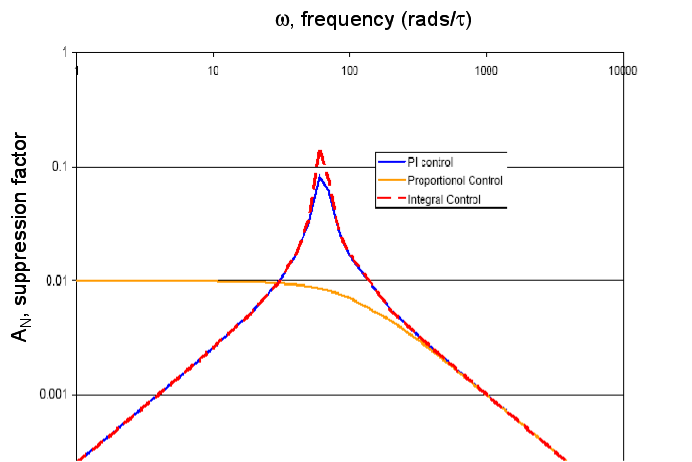
\includegraphics[width=0.6\textwidth]{pics/PI_noise_suppression}
\end{center}
Comparison of the suppression factor, $A_N$, for different feedback schemes. The feedback control loop parameters are $g_P = -100$ and $g_I = -4000$.
\end{frame}

\end{document}
